\documentclass{article}
\usepackage{amsmath, amssymb}
\usepackage{bm}
\usepackage{graphicx} % Required for inserting images
\usepackage{tikz}
\usepackage{float}
\usepackage[round]{natbib}

\bibliographystyle{plainnat}
\usepackage[a4paper, top = 3cm,
                     bottom = 3cm,
                     left = 3cm,
                     right = 3cm]{geometry}


\title{Conservation and harvesting in endogenous ecological networks}
\author{Simon Jean}
\date{January 2024}


%%%%%%%%%%%%%%%%%%%%%%
\newcommand*{\xMin}{0}%
\newcommand*{\xMax}{5}%
\newcommand*{\yMin}{0}%
\newcommand*{\yMax}{3}%


\newtheorem{assumption}{Assumption}

\begin{document}
\maketitle

\begin{itemize}
\item IPBES or something about the importance of non human species for ecosystem services etc
\item Management regards decisions concerning conservation and harvesting in ecological networks
\item Non human populations are spatially distributed
\item Considering the spatial layer is paramount in managing the flows of ecosystem services provided by ecological resources
\item Understanding how to shape ecological networks where resources are harvested to maximize conservation measures is key
\item Dispersal is a public good feature : the current flow of benefits in a patch depends on the decisions of all other landowners
\item This article is concerned with the ecological economic network structures emerging from various conservation objectives. 
\item It characterizes, using dynamic programming and network theory, the properties of optimal networks, as well as non cooperative networks. 
\item 
\end{itemize}


\section{Model}
\subsection{Economic and ecological submodels}
I model an ecological network as a meta-population model with $N$ patches, with $N$ distinct landowners. In each patch, population grows depending on patch specific characteristics, and the initial size at the beginning of period $t$. 

In each period and each patch, landowners derive a flow of benefits from harvesting the resource, and harvest down to a residual stock $e_{it} = X_{it}-h_{it}$, with net marginal benefit $b_i(X_{it}-e_{it})$, where $b_i()>0$ and $b'_i()\leq 0$.

 Once the resource has grown, it disperses through space. Dispersal depends on immuable factors (altitude differential, ruggedness...) and endogenous factors, including relative densities (e.g. between patch $i$ and patch $j$, migration depends on $X_{it}$ and $X_{jt}$) and devices that can increase or reduce inbound or outbound connectivity. To keep things tractable and stylized, assume a landowner can fence its land ($z_{it}^F$) or create ecoducts/ bait ($z^B_{it}$). Dispersal between two patches depends on relative densities, the amount of fencing and baiting, as well as the immutable factors \footnote{Note that $d_{ijt} \neq d_{jit}$ in general.} : 

\begin{align}
d_{ij, t+1} &\in [\underline{d_{ij}}, \bar{d_{ij}}] \subset [0,1] \\
d_{ij, t+1} & = d_{ij, t+1}\left(z_{it}^F, z_{jt}^B, X_{it}, X_{jt}; d_{ijt}\right)
\label{eq:dispersal}
\end{align}


The timing of the model is illustrated in figure \ref{fig:timing}. Overall, the population stock in patch $i$ in period $t+1$ is such that : 
\begin{equation}
X_{i,t+1} = \sum_{i=1}^N d_{ji,t+1}\left(z_j^F, z_i^B, X_i, X_j; d_{ijt}\right) g_j(e_{jt})
\end{equation}

In each period, a landowner maximizes the following payoff : 

\begin{equation}
\Pi_{it} = \int_{X_{it}}^{e_{it}} b(x)dx - c_{iF}(z_{it}^F) - c_{iB}(z_{it}^B)
\end{equation}

\subsubsection{Graph theoretical apparatus}

\begin{itemize}
\item Vertices are patches
\item For each node $i$, there is an edge to patch $j$ if $d_{ijt}>0$ : if there is an outbound connection to $j$.  
\item The weight
\end{itemize}

\subsection{Objectives for a conservatonists}

A conservationist can be interested in several dimensions of conservation. 
First, it can want to maximize the population size in each period (idea is welfare is increasing in the number of animals, maybe their own welfare) : 

\begin{equation}
S(X) = \sum_{i=1}^N X_{it}
\end{equation} 

Second, a conservationist can care about the aggregate fragility of the ecosystem : 
\begin{itemize}
\item Spatial distribution of stock
\item Mean and variance of inbound and outbound degrees?
\item Weighted degrees, and their distribution
\end{itemize}

Third, cares about a resilience potential : 

\section{Model}
\begin{itemize}
\item Find dynamic Nash Equilibrium
\item Maximize the sum of profits
\item Maximize the sum of profits and conservation function
\end{itemize}
Goal is to find a graph theory statistic link. 

\section{Numerical Illustration}


\section{Conclusion}

\newpage
\begin{figure}[H]
  \centering
  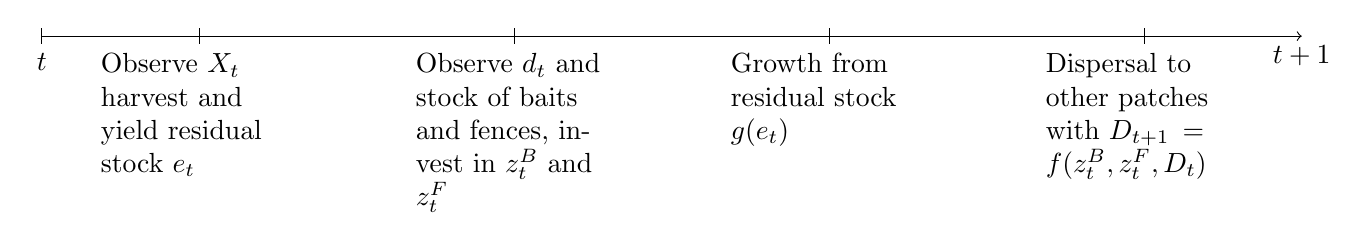
\begin{tikzpicture}
    % Draw the arrow
    \draw[->] (0,0) -- (16,0) node[anchor=north] {$t+1$};
    % Draw ticks and labels
    \draw (0, .1)--(0,-.1) node[anchor = north]{$t$};
    \draw (2, .1)--(2,-.1) node[anchor = north, text width = 2.5cm]{Observe $X_t$ harvest and yield residual stock $e_t$};
    \draw (6, .1)--(6,-.1) node[anchor = north, text width = 2.5cm] {Observe $d_t$ and stock of baits and fences, invest in $z_t^B$ and $z_t^F$};
    \draw (10, .1)--(10,-.1) node[anchor = north, text width = 2.5cm]{Growth from residual stock $g(e_t)$};
    \draw (14,.1)--(14,-.1) node[anchor = north, text width = 2.5cm]{Dispersal to other patches with $D_{t+1}=f(z_t^B, z_t^F, D_t)$};
  \end{tikzpicture}
  \caption{Timing of the model}
  \label{fig:timing}
\end{figure}



\end{document}